\documentclass[border=10pt]{standalone}
\usepackage{tikz}
\usetikzlibrary{calc,positioning,shadows.blur,decorations.pathreplacing}
\usepackage{etoolbox}
\usepackage{graphicx}
\usepackage{amsmath}
\graphicspath{{/home/jake/Documents/MOSES/MCOR/python/}}

\begin{document}
	\begin{tikzpicture}
	
	%begin by adding a node for each figure
	\node[inner sep=0pt] (fig1) at (0,0)
		{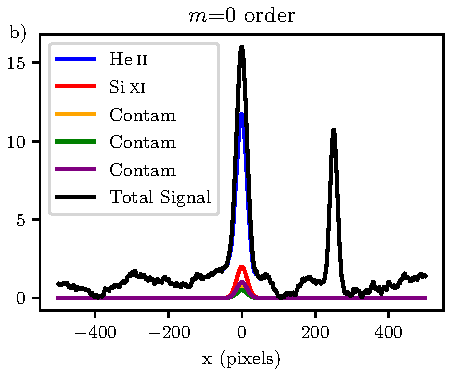
\includegraphics[width=.25\textwidth]{fig1}};
	\node[inner sep=0pt] (fig2) at (4,0)
		{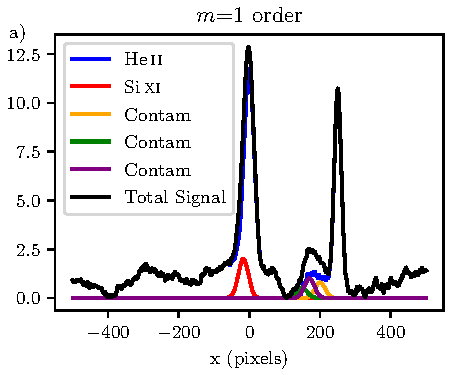
\includegraphics[width=.25\textwidth]{fig2}};
	\node[inner sep=0pt] (fig3) at (-4,0)
		{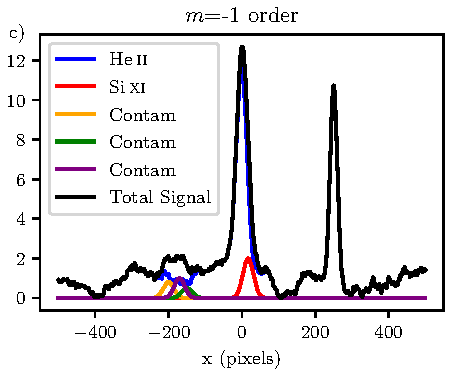
\includegraphics[width=.25\textwidth]{fig3}};
	\node[inner sep=0pt] (fig4) at (-2,-3)
		{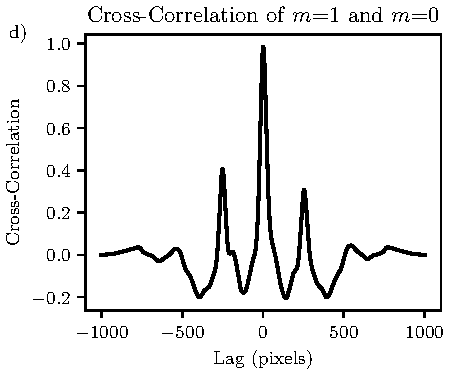
\includegraphics[width=.25\textwidth]{fig4}};
	\node[inner sep=0pt] (fig5) at (2,-3)
		{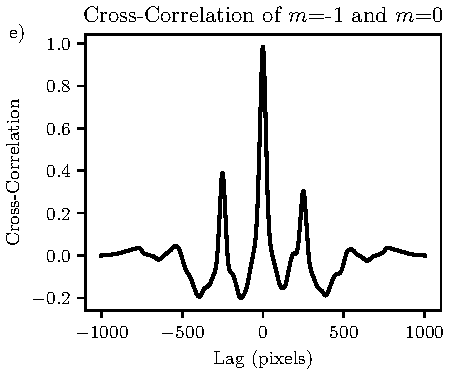
\includegraphics[width=.25\textwidth]{fig5}};
	\node[inner sep=0pt] (fig6) at (4,-6)
		{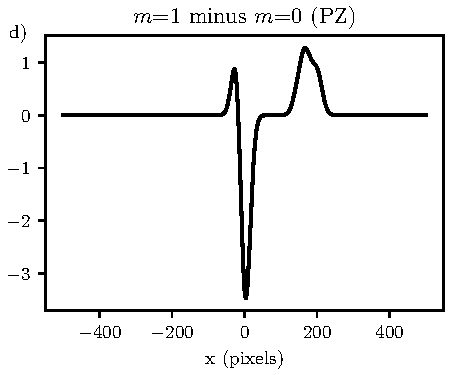
\includegraphics[width=.25\textwidth]{fig6}};
	\node[inner sep=0pt] (fig7) at (-4,-6)
		{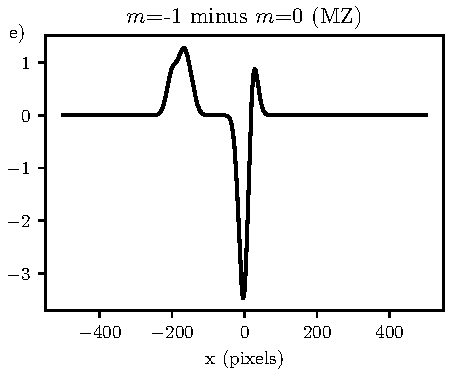
\includegraphics[width=.25\textwidth]{fig7}};
	\node[inner sep=0pt] (fig8) at (0,-7)
		{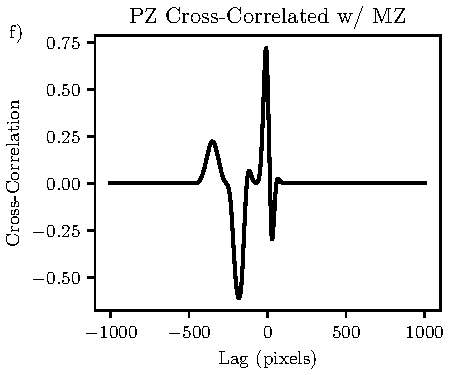
\includegraphics[width=.25\textwidth]{fig8}};
		
	%add symbol for operation
	\node[inner sep=0pt](cc1) at (2,-1.5)
		{$\bigotimes$};
	\node[inner sep=0pt](cc2) at (-2,-1.5)
		{$\bigotimes$};
	\node[inner sep=1pt](dif1) at (4,-4.5)
		{$\boldsymbol{\bigtriangleup}$};
	\node[inner sep=1pt](dif2) at (-4,-4.5)
		{$\boldsymbol{\bigtriangleup}$};
	\node[inner sep=0pt](cc3) at (0,-5.4)
		{$\bigotimes$};
	\node[inner sep=0pt](mid) at (0,-4.5)
		{};
	
		
		
	%lets try drawing some lines between them.
	\draw[->] (fig1.south east) -- (cc1.north west);
	\draw[->] (fig2.south west) -- (cc1.north east);
	\draw[->] (cc1.south) -- (fig5.north);
	
	\draw[->] (fig1.south west) -- (cc2.north east);
	\draw[->] (fig3.south east) -- (cc2.north west);
	\draw[->] (cc2.south) -- (fig4.north);
	
	\draw[->] (fig2.south) -- (dif1.north);
	\draw[->] (fig3.south) -- (dif2.north);
	\draw[-] (fig1.south) -- (mid);
	\draw[->] (mid) -- (dif1.west);
	\draw[->] (mid) -- (dif2.east);
	\draw[->] (dif2.south) -- (fig7.north);
	\draw[->] (dif1.south) -- (fig6.north);
	
	\draw[->] (-2.5,-5.4) -- (cc3.west);
	\draw[->] (2.5,-5.4) -- (cc3.east);
	\draw[->] (cc3.south) -- (fig8.north);
	
	%draw a symbol legend
	\node(align)[draw, rotate=90] at (-5,-3) {
		\begin{tabular}{c}
			\tiny{$\bigotimes$ = Cross Correlation} \\
			\tiny{$\boldsymbol{\bigtriangleup}$ = Difference}
		\end{tabular}};
	

	\end{tikzpicture}
\end{document}